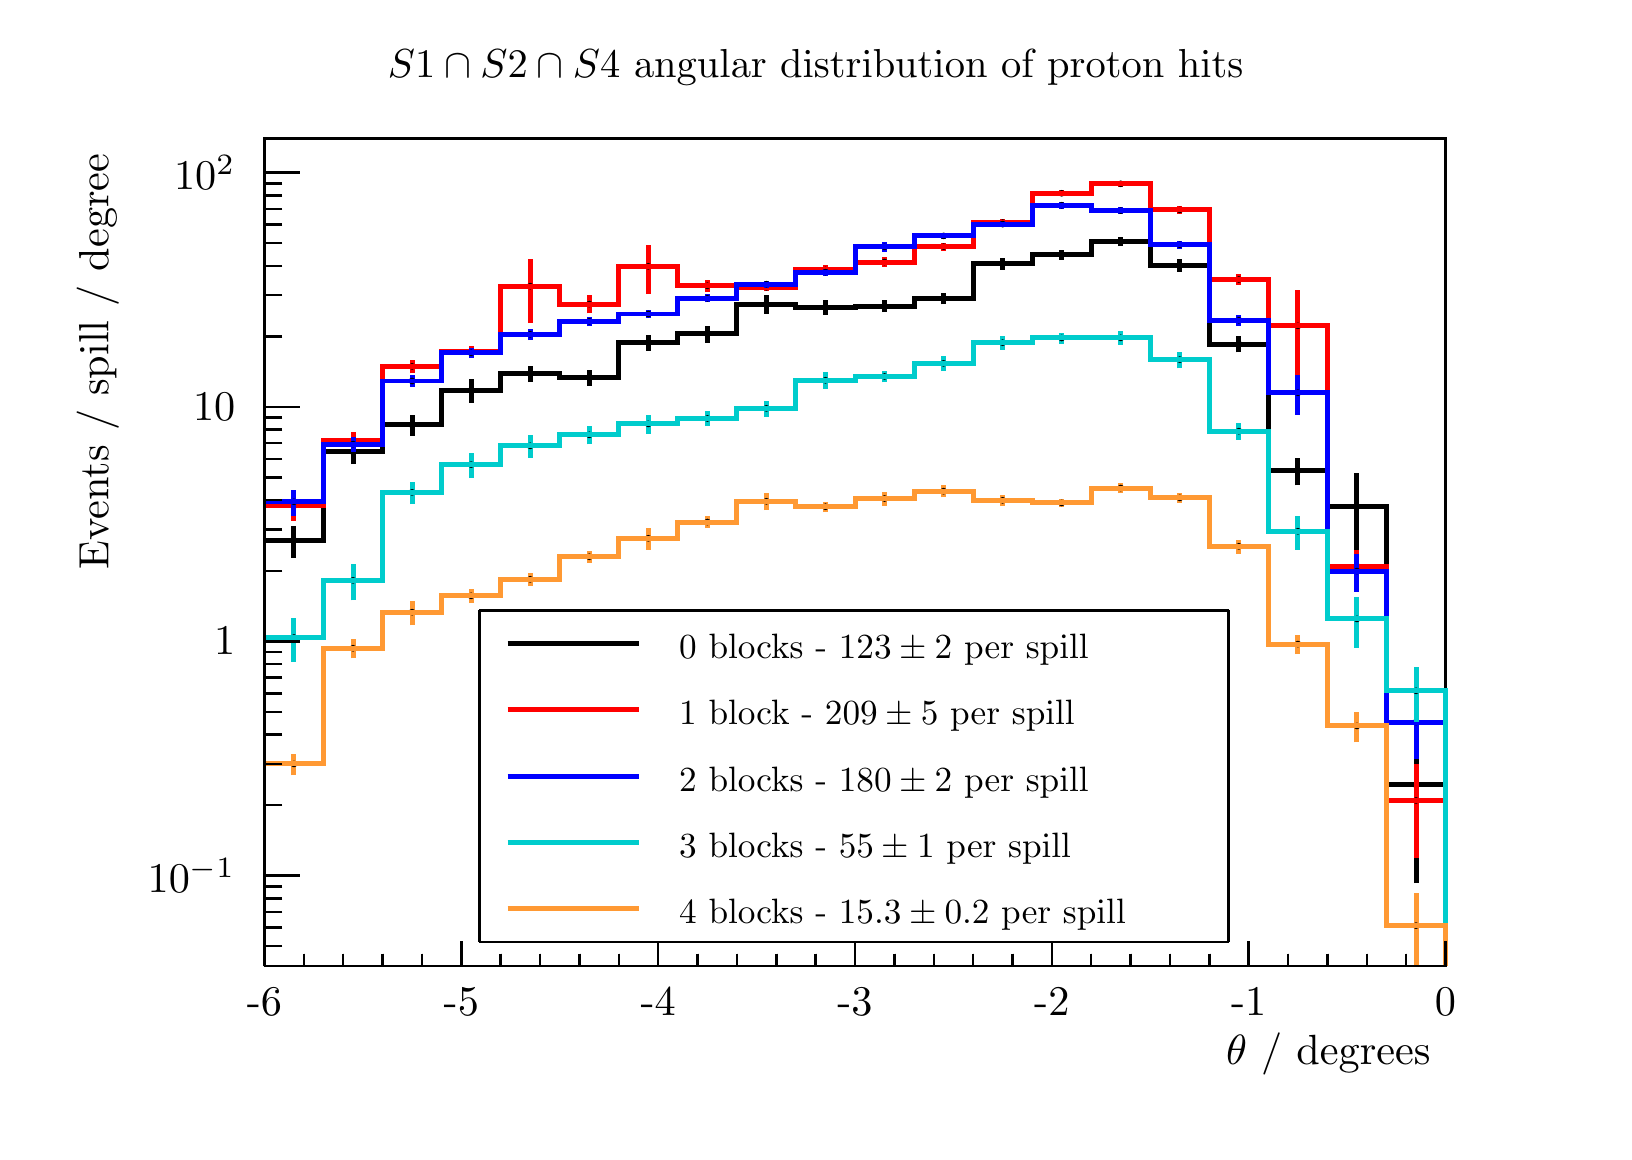
\begin{tikzpicture}
\pgfdeclareplotmark{cross} {
\pgfpathmoveto{\pgfpoint{-0.3\pgfplotmarksize}{\pgfplotmarksize}}
\pgfpathlineto{\pgfpoint{+0.3\pgfplotmarksize}{\pgfplotmarksize}}
\pgfpathlineto{\pgfpoint{+0.3\pgfplotmarksize}{0.3\pgfplotmarksize}}
\pgfpathlineto{\pgfpoint{+1\pgfplotmarksize}{0.3\pgfplotmarksize}}
\pgfpathlineto{\pgfpoint{+1\pgfplotmarksize}{-0.3\pgfplotmarksize}}
\pgfpathlineto{\pgfpoint{+0.3\pgfplotmarksize}{-0.3\pgfplotmarksize}}
\pgfpathlineto{\pgfpoint{+0.3\pgfplotmarksize}{-1.\pgfplotmarksize}}
\pgfpathlineto{\pgfpoint{-0.3\pgfplotmarksize}{-1.\pgfplotmarksize}}
\pgfpathlineto{\pgfpoint{-0.3\pgfplotmarksize}{-0.3\pgfplotmarksize}}
\pgfpathlineto{\pgfpoint{-1.\pgfplotmarksize}{-0.3\pgfplotmarksize}}
\pgfpathlineto{\pgfpoint{-1.\pgfplotmarksize}{0.3\pgfplotmarksize}}
\pgfpathlineto{\pgfpoint{-0.3\pgfplotmarksize}{0.3\pgfplotmarksize}}
\pgfpathclose
\pgfusepathqstroke
}
\pgfdeclareplotmark{cross*} {
\pgfpathmoveto{\pgfpoint{-0.3\pgfplotmarksize}{\pgfplotmarksize}}
\pgfpathlineto{\pgfpoint{+0.3\pgfplotmarksize}{\pgfplotmarksize}}
\pgfpathlineto{\pgfpoint{+0.3\pgfplotmarksize}{0.3\pgfplotmarksize}}
\pgfpathlineto{\pgfpoint{+1\pgfplotmarksize}{0.3\pgfplotmarksize}}
\pgfpathlineto{\pgfpoint{+1\pgfplotmarksize}{-0.3\pgfplotmarksize}}
\pgfpathlineto{\pgfpoint{+0.3\pgfplotmarksize}{-0.3\pgfplotmarksize}}
\pgfpathlineto{\pgfpoint{+0.3\pgfplotmarksize}{-1.\pgfplotmarksize}}
\pgfpathlineto{\pgfpoint{-0.3\pgfplotmarksize}{-1.\pgfplotmarksize}}
\pgfpathlineto{\pgfpoint{-0.3\pgfplotmarksize}{-0.3\pgfplotmarksize}}
\pgfpathlineto{\pgfpoint{-1.\pgfplotmarksize}{-0.3\pgfplotmarksize}}
\pgfpathlineto{\pgfpoint{-1.\pgfplotmarksize}{0.3\pgfplotmarksize}}
\pgfpathlineto{\pgfpoint{-0.3\pgfplotmarksize}{0.3\pgfplotmarksize}}
\pgfpathclose
\pgfusepathqfillstroke
}
\pgfdeclareplotmark{newstar} {
\pgfpathmoveto{\pgfqpoint{0pt}{\pgfplotmarksize}}
\pgfpathlineto{\pgfqpointpolar{44}{0.5\pgfplotmarksize}}
\pgfpathlineto{\pgfqpointpolar{18}{\pgfplotmarksize}}
\pgfpathlineto{\pgfqpointpolar{-20}{0.5\pgfplotmarksize}}
\pgfpathlineto{\pgfqpointpolar{-54}{\pgfplotmarksize}}
\pgfpathlineto{\pgfqpointpolar{-90}{0.5\pgfplotmarksize}}
\pgfpathlineto{\pgfqpointpolar{234}{\pgfplotmarksize}}
\pgfpathlineto{\pgfqpointpolar{198}{0.5\pgfplotmarksize}}
\pgfpathlineto{\pgfqpointpolar{162}{\pgfplotmarksize}}
\pgfpathlineto{\pgfqpointpolar{134}{0.5\pgfplotmarksize}}
\pgfpathclose
\pgfusepathqstroke
}
\pgfdeclareplotmark{newstar*} {
\pgfpathmoveto{\pgfqpoint{0pt}{\pgfplotmarksize}}
\pgfpathlineto{\pgfqpointpolar{44}{0.5\pgfplotmarksize}}
\pgfpathlineto{\pgfqpointpolar{18}{\pgfplotmarksize}}
\pgfpathlineto{\pgfqpointpolar{-20}{0.5\pgfplotmarksize}}
\pgfpathlineto{\pgfqpointpolar{-54}{\pgfplotmarksize}}
\pgfpathlineto{\pgfqpointpolar{-90}{0.5\pgfplotmarksize}}
\pgfpathlineto{\pgfqpointpolar{234}{\pgfplotmarksize}}
\pgfpathlineto{\pgfqpointpolar{198}{0.5\pgfplotmarksize}}
\pgfpathlineto{\pgfqpointpolar{162}{\pgfplotmarksize}}
\pgfpathlineto{\pgfqpointpolar{134}{0.5\pgfplotmarksize}}
\pgfpathclose
\pgfusepathqfillstroke
}
\definecolor{c}{rgb}{1,1,1};
\draw [color=c, fill=c] (0,0) rectangle (20,14.0115);
\draw [color=c, fill=c] (3,2.10172) rectangle (18,12.6103);
\definecolor{c}{rgb}{0,0,0};
\draw [c,line width=0.9] (3,2.10172) -- (3,12.6103) -- (18,12.6103) -- (18,2.10172) -- (3,2.10172);
\definecolor{c}{rgb}{1,1,1};
\draw [color=c, fill=c] (3,2.10172) rectangle (18,12.6103);
\definecolor{c}{rgb}{0,0,0};
\draw [c,line width=0.9] (3,2.10172) -- (3,12.6103) -- (18,12.6103) -- (18,2.10172) -- (3,2.10172);
\definecolor{c}{rgb}{0,0,0.6};
\draw [c,line width=0.9] (3,2.10172) -- (3.75,2.10172) -- (3.75,2.10172) -- (4.5,2.10172) -- (4.5,2.10172) -- (5.25,2.10172) -- (5.25,2.10172) -- (6,2.10172) -- (6,2.10172) -- (6.75,2.10172) -- (6.75,2.10172) -- (7.5,2.10172) -- (7.5,2.10172) --
 (8.25,2.10172) -- (8.25,2.10172) -- (9,2.10172) -- (9,2.10172) -- (9.75,2.10172) -- (9.75,2.10172) -- (10.5,2.10172) -- (10.5,2.10172) -- (11.25,2.10172) -- (11.25,2.10172) -- (12,2.10172) -- (12,2.10172) -- (12.75,2.10172) -- (12.75,2.10172) --
 (13.5,2.10172) -- (13.5,2.10172) -- (14.25,2.10172) -- (14.25,2.10172) -- (15,2.10172) -- (15,2.10172) -- (15.75,2.10172) -- (15.75,2.10172) -- (16.5,2.10172) -- (16.5,2.10172) -- (17.25,2.10172) -- (17.25,2.10172) -- (18,2.10172) -- (18,2.10172);
\definecolor{c}{rgb}{0,0,0};
\draw [c,line width=0.9] (3,2.10172) -- (18,2.10172);
\draw [c,line width=0.9] (3,2.41698) -- (3,2.10172);
\draw [c,line width=0.9] (3.5,2.25935) -- (3.5,2.10172);
\draw [c,line width=0.9] (4,2.25935) -- (4,2.10172);
\draw [c,line width=0.9] (4.5,2.25935) -- (4.5,2.10172);
\draw [c,line width=0.9] (5,2.25935) -- (5,2.10172);
\draw [c,line width=0.9] (5.5,2.41698) -- (5.5,2.10172);
\draw [c,line width=0.9] (6,2.25935) -- (6,2.10172);
\draw [c,line width=0.9] (6.5,2.25935) -- (6.5,2.10172);
\draw [c,line width=0.9] (7,2.25935) -- (7,2.10172);
\draw [c,line width=0.9] (7.5,2.25935) -- (7.5,2.10172);
\draw [c,line width=0.9] (8,2.41698) -- (8,2.10172);
\draw [c,line width=0.9] (8.5,2.25935) -- (8.5,2.10172);
\draw [c,line width=0.9] (9,2.25935) -- (9,2.10172);
\draw [c,line width=0.9] (9.5,2.25935) -- (9.5,2.10172);
\draw [c,line width=0.9] (10,2.25935) -- (10,2.10172);
\draw [c,line width=0.9] (10.5,2.41698) -- (10.5,2.10172);
\draw [c,line width=0.9] (11,2.25935) -- (11,2.10172);
\draw [c,line width=0.9] (11.5,2.25935) -- (11.5,2.10172);
\draw [c,line width=0.9] (12,2.25935) -- (12,2.10172);
\draw [c,line width=0.9] (12.5,2.25935) -- (12.5,2.10172);
\draw [c,line width=0.9] (13,2.41698) -- (13,2.10172);
\draw [c,line width=0.9] (13.5,2.25935) -- (13.5,2.10172);
\draw [c,line width=0.9] (14,2.25935) -- (14,2.10172);
\draw [c,line width=0.9] (14.5,2.25935) -- (14.5,2.10172);
\draw [c,line width=0.9] (15,2.25935) -- (15,2.10172);
\draw [c,line width=0.9] (15.5,2.41698) -- (15.5,2.10172);
\draw [c,line width=0.9] (16,2.25935) -- (16,2.10172);
\draw [c,line width=0.9] (16.5,2.25935) -- (16.5,2.10172);
\draw [c,line width=0.9] (17,2.25935) -- (17,2.10172);
\draw [c,line width=0.9] (17.5,2.25935) -- (17.5,2.10172);
\draw [c,line width=0.9] (18,2.41698) -- (18,2.10172);
\draw [anchor=base] (3,1.4712) node[scale=1.52731, color=c, rotate=0]{-6};
\draw [anchor=base] (5.5,1.4712) node[scale=1.52731, color=c, rotate=0]{-5};
\draw [anchor=base] (8,1.4712) node[scale=1.52731, color=c, rotate=0]{-4};
\draw [anchor=base] (10.5,1.4712) node[scale=1.52731, color=c, rotate=0]{-3};
\draw [anchor=base] (13,1.4712) node[scale=1.52731, color=c, rotate=0]{-2};
\draw [anchor=base] (15.5,1.4712) node[scale=1.52731, color=c, rotate=0]{-1};
\draw [anchor=base] (18,1.4712) node[scale=1.52731, color=c, rotate=0]{0};
\draw [anchor= east] (18,0.980802) node[scale=1.52731, color=c, rotate=0]{$\theta$ / degrees};
\draw [c,line width=0.9] (3,2.10172) -- (3,12.6103);
\draw [c,line width=0.9] (3.225,2.35317) -- (3,2.35317);
\draw [c,line width=0.9] (3.225,2.58883) -- (3,2.58883);
\draw [c,line width=0.9] (3.225,2.78809) -- (3,2.78809);
\draw [c,line width=0.9] (3.225,2.96069) -- (3,2.96069);
\draw [c,line width=0.9] (3.225,3.11293) -- (3,3.11293);
\draw [c,line width=0.9] (3.45,3.24912) -- (3,3.24912);
\draw [anchor= east] (2.82,3.24912) node[scale=1.52731, color=c, rotate=0]{$10^{-1}$};
\draw [c,line width=0.9] (3.225,4.14507) -- (3,4.14507);
\draw [c,line width=0.9] (3.225,4.66916) -- (3,4.66916);
\draw [c,line width=0.9] (3.225,5.04101) -- (3,5.04101);
\draw [c,line width=0.9] (3.225,5.32945) -- (3,5.32945);
\draw [c,line width=0.9] (3.225,5.56511) -- (3,5.56511);
\draw [c,line width=0.9] (3.225,5.76436) -- (3,5.76436);
\draw [c,line width=0.9] (3.225,5.93696) -- (3,5.93696);
\draw [c,line width=0.9] (3.225,6.08921) -- (3,6.08921);
\draw [c,line width=0.9] (3.45,6.22539) -- (3,6.22539);
\draw [anchor= east] (2.82,6.22539) node[scale=1.52731, color=c, rotate=0]{1};
\draw [c,line width=0.9] (3.225,7.12134) -- (3,7.12134);
\draw [c,line width=0.9] (3.225,7.64544) -- (3,7.64544);
\draw [c,line width=0.9] (3.225,8.01729) -- (3,8.01729);
\draw [c,line width=0.9] (3.225,8.30572) -- (3,8.30572);
\draw [c,line width=0.9] (3.225,8.54139) -- (3,8.54139);
\draw [c,line width=0.9] (3.225,8.74064) -- (3,8.74064);
\draw [c,line width=0.9] (3.225,8.91324) -- (3,8.91324);
\draw [c,line width=0.9] (3.225,9.06548) -- (3,9.06548);
\draw [c,line width=0.9] (3.45,9.20167) -- (3,9.20167);
\draw [anchor= east] (2.82,9.20167) node[scale=1.52731, color=c, rotate=0]{10};
\draw [c,line width=0.9] (3.225,10.0976) -- (3,10.0976);
\draw [c,line width=0.9] (3.225,10.6217) -- (3,10.6217);
\draw [c,line width=0.9] (3.225,10.9936) -- (3,10.9936);
\draw [c,line width=0.9] (3.225,11.282) -- (3,11.282);
\draw [c,line width=0.9] (3.225,11.5177) -- (3,11.5177);
\draw [c,line width=0.9] (3.225,11.7169) -- (3,11.7169);
\draw [c,line width=0.9] (3.225,11.8895) -- (3,11.8895);
\draw [c,line width=0.9] (3.225,12.0418) -- (3,12.0418);
\draw [c,line width=0.9] (3.45,12.1779) -- (3,12.1779);
\draw [anchor= east] (2.82,12.1779) node[scale=1.52731, color=c, rotate=0]{$10^{2}$};
\draw [anchor= east] (0.882522,12.6103) node[scale=1.52731, color=c, rotate=90]{ Events / spill / degree};
\draw [c,line width=1.8] (3.375,7.28949) -- (3.375,7.50668);
\draw [c,line width=1.8] (3.375,7.50668) -- (3.375,7.69257);
\foreach \P in {(3.375,7.50668)}{\draw[mark options={color=c,fill=c},mark size=2.402402pt,mark=*,mark size=1pt] plot coordinates {\P};}
\draw [c,line width=1.8] (4.125,8.47394) -- (4.125,8.63233);
\draw [c,line width=1.8] (4.125,8.63233) -- (4.125,8.77341);
\foreach \P in {(4.125,8.63233)}{\draw[mark options={color=c,fill=c},mark size=2.402402pt,mark=*,mark size=1pt] plot coordinates {\P};}
\draw [c,line width=1.8] (4.875,8.83354) -- (4.875,8.97497);
\draw [c,line width=1.8] (4.875,8.97497) -- (4.875,9.10244);
\foreach \P in {(4.875,8.97497)}{\draw[mark options={color=c,fill=c},mark size=2.402402pt,mark=*,mark size=1pt] plot coordinates {\P};}
\draw [c,line width=1.8] (5.625,9.25194) -- (5.625,9.41363);
\draw [c,line width=1.8] (5.625,9.41363) -- (5.625,9.55733);
\foreach \P in {(5.625,9.41363)}{\draw[mark options={color=c,fill=c},mark size=2.402402pt,mark=*,mark size=1pt] plot coordinates {\P};}
\draw [c,line width=1.8] (6.375,9.51761) -- (6.375,9.62374);
\draw [c,line width=1.8] (6.375,9.62374) -- (6.375,9.7218);
\foreach \P in {(6.375,9.62374)}{\draw[mark options={color=c,fill=c},mark size=2.402402pt,mark=*,mark size=1pt] plot coordinates {\P};}
\draw [c,line width=1.8] (7.125,9.46933) -- (7.125,9.57675);
\draw [c,line width=1.8] (7.125,9.57675) -- (7.125,9.67592);
\foreach \P in {(7.125,9.57675)}{\draw[mark options={color=c,fill=c},mark size=2.402402pt,mark=*,mark size=1pt] plot coordinates {\P};}
\draw [c,line width=1.8] (7.875,9.91828) -- (7.875,10.0227);
\draw [c,line width=1.8] (7.875,10.0227) -- (7.875,10.1194);
\foreach \P in {(7.875,10.0227)}{\draw[mark options={color=c,fill=c},mark size=2.402402pt,mark=*,mark size=1pt] plot coordinates {\P};}
\draw [c,line width=1.8] (8.625,10.0157) -- (8.625,10.13);
\draw [c,line width=1.8] (8.625,10.13) -- (8.625,10.2351);
\foreach \P in {(8.625,10.13)}{\draw[mark options={color=c,fill=c},mark size=2.402402pt,mark=*,mark size=1pt] plot coordinates {\P};}
\draw [c,line width=1.8] (9.375,10.3821) -- (9.375,10.5089);
\draw [c,line width=1.8] (9.375,10.5089) -- (9.375,10.6243);
\foreach \P in {(9.375,10.5089)}{\draw[mark options={color=c,fill=c},mark size=2.402402pt,mark=*,mark size=1pt] plot coordinates {\P};}
\draw [c,line width=1.8] (10.125,10.3741) -- (10.125,10.4697);
\draw [c,line width=1.8] (10.125,10.4697) -- (10.125,10.5587);
\foreach \P in {(10.125,10.4697)}{\draw[mark options={color=c,fill=c},mark size=2.402402pt,mark=*,mark size=1pt] plot coordinates {\P};}
\draw [c,line width=1.8] (10.875,10.405) -- (10.875,10.4816);
\draw [c,line width=1.8] (10.875,10.4816) -- (10.875,10.5539);
\foreach \P in {(10.875,10.4816)}{\draw[mark options={color=c,fill=c},mark size=2.402402pt,mark=*,mark size=1pt] plot coordinates {\P};}
\draw [c,line width=1.8] (11.625,10.505) -- (11.625,10.5816);
\draw [c,line width=1.8] (11.625,10.5816) -- (11.625,10.6539);
\foreach \P in {(11.625,10.5816)}{\draw[mark options={color=c,fill=c},mark size=2.402402pt,mark=*,mark size=1pt] plot coordinates {\P};}
\draw [c,line width=1.8] (12.375,10.9417) -- (12.375,11.0213);
\draw [c,line width=1.8] (12.375,11.0213) -- (12.375,11.0963);
\foreach \P in {(12.375,11.0213)}{\draw[mark options={color=c,fill=c},mark size=2.402402pt,mark=*,mark size=1pt] plot coordinates {\P};}
\draw [c,line width=1.8] (13.125,11.0726) -- (13.125,11.1364);
\draw [c,line width=1.8] (13.125,11.1364) -- (13.125,11.1973);
\foreach \P in {(13.125,11.1364)}{\draw[mark options={color=c,fill=c},mark size=2.402402pt,mark=*,mark size=1pt] plot coordinates {\P};}
\draw [c,line width=1.8] (13.875,11.2439) -- (13.875,11.3002);
\draw [c,line width=1.8] (13.875,11.3002) -- (13.875,11.3541);
\foreach \P in {(13.875,11.3002)}{\draw[mark options={color=c,fill=c},mark size=2.402402pt,mark=*,mark size=1pt] plot coordinates {\P};}
\draw [c,line width=1.8] (14.625,10.9204) -- (14.625,11.0001);
\draw [c,line width=1.8] (14.625,11.0001) -- (14.625,11.0752);
\foreach \P in {(14.625,11.0001)}{\draw[mark options={color=c,fill=c},mark size=2.402402pt,mark=*,mark size=1pt] plot coordinates {\P};}
\draw [c,line width=1.8] (15.375,9.8936) -- (15.375,9.99999);
\draw [c,line width=1.8] (15.375,9.99999) -- (15.375,10.0983);
\foreach \P in {(15.375,9.99999)}{\draw[mark options={color=c,fill=c},mark size=2.402402pt,mark=*,mark size=1pt] plot coordinates {\P};}
\draw [c,line width=1.8] (16.125,8.20514) -- (16.125,8.3932);
\draw [c,line width=1.8] (16.125,8.3932) -- (16.125,8.55734);
\foreach \P in {(16.125,8.3932)}{\draw[mark options={color=c,fill=c},mark size=2.402402pt,mark=*,mark size=1pt] plot coordinates {\P};}
\draw [c,line width=1.8] (16.875,7.28862) -- (16.875,7.93686);
\draw [c,line width=1.8] (16.875,7.93686) -- (16.875,8.36658);
\foreach \P in {(16.875,7.93686)}{\draw[mark options={color=c,fill=c},mark size=2.402402pt,mark=*,mark size=1pt] plot coordinates {\P};}
\draw [c,line width=1.8] (17.625,3.15452) -- (17.625,4.40082);
\draw [c,line width=1.8] (17.625,4.40082) -- (17.625,5.02336);
\foreach \P in {(17.625,4.40082)}{\draw[mark options={color=c,fill=c},mark size=2.402402pt,mark=*,mark size=1pt] plot coordinates {\P};}
\draw [c,line width=1.8] (3,7.50668) -- (3.75,7.50668) -- (3.75,8.63233) -- (4.5,8.63233) -- (4.5,8.97497) -- (5.25,8.97497) -- (5.25,9.41363) -- (6,9.41363) -- (6,9.62374) -- (6.75,9.62374) -- (6.75,9.57675) -- (7.5,9.57675) -- (7.5,10.0227) --
 (8.25,10.0227) -- (8.25,10.13) -- (9,10.13) -- (9,10.5089) -- (9.75,10.5089) -- (9.75,10.4697) -- (10.5,10.4697) -- (10.5,10.4816) -- (11.25,10.4816) -- (11.25,10.5816) -- (12,10.5816) -- (12,11.0213) -- (12.75,11.0213) -- (12.75,11.1364) --
 (13.5,11.1364) -- (13.5,11.3002) -- (14.25,11.3002) -- (14.25,11.0001) -- (15,11.0001) -- (15,9.99999) -- (15.75,9.99999) -- (15.75,8.3932) -- (16.5,8.3932) -- (16.5,7.93686) -- (17.25,7.93686) -- (17.25,4.40082) -- (18,4.40082) -- (18,2.10172);
\definecolor{c}{rgb}{1,0,0};
\draw [c,line width=1.8] (3.375,7.75388) -- (3.375,7.94795);
\draw [c,line width=1.8] (3.375,7.94795) -- (3.375,8.11664);
\definecolor{c}{rgb}{0,0,0};
\foreach \P in {(3.375,7.94795)}{\draw[mark options={color=c,fill=c},mark size=2.402402pt,mark=*,mark size=1pt] plot coordinates {\P};}
\definecolor{c}{rgb}{1,0,0};
\draw [c,line width=1.8] (4.125,8.64419) -- (4.125,8.77001);
\draw [c,line width=1.8] (4.125,8.77001) -- (4.125,8.88466);
\definecolor{c}{rgb}{0,0,0};
\foreach \P in {(4.125,8.77001)}{\draw[mark options={color=c,fill=c},mark size=2.402402pt,mark=*,mark size=1pt] plot coordinates {\P};}
\definecolor{c}{rgb}{1,0,0};
\draw [c,line width=1.8] (4.875,9.62858) -- (4.875,9.71635);
\draw [c,line width=1.8] (4.875,9.71635) -- (4.875,9.79853);
\definecolor{c}{rgb}{0,0,0};
\foreach \P in {(4.875,9.71635)}{\draw[mark options={color=c,fill=c},mark size=2.402402pt,mark=*,mark size=1pt] plot coordinates {\P};}
\definecolor{c}{rgb}{1,0,0};
\draw [c,line width=1.8] (5.625,9.82455) -- (5.625,9.90121);
\draw [c,line width=1.8] (5.625,9.90121) -- (5.625,9.97357);
\definecolor{c}{rgb}{0,0,0};
\foreach \P in {(5.625,9.90121)}{\draw[mark options={color=c,fill=c},mark size=2.402402pt,mark=*,mark size=1pt] plot coordinates {\P};}
\definecolor{c}{rgb}{1,0,0};
\draw [c,line width=1.8] (6.375,10.2657) -- (6.375,10.7355);
\draw [c,line width=1.8] (6.375,10.7355) -- (6.375,11.0794);
\definecolor{c}{rgb}{0,0,0};
\foreach \P in {(6.375,10.7355)}{\draw[mark options={color=c,fill=c},mark size=2.402402pt,mark=*,mark size=1pt] plot coordinates {\P};}
\definecolor{c}{rgb}{1,0,0};
\draw [c,line width=1.8] (7.125,10.3887) -- (7.125,10.508);
\draw [c,line width=1.8] (7.125,10.508) -- (7.125,10.6173);
\definecolor{c}{rgb}{0,0,0};
\foreach \P in {(7.125,10.508)}{\draw[mark options={color=c,fill=c},mark size=2.402402pt,mark=*,mark size=1pt] plot coordinates {\P};}
\definecolor{c}{rgb}{1,0,0};
\draw [c,line width=1.8] (7.875,10.6346) -- (7.875,10.9875);
\draw [c,line width=1.8] (7.875,10.9875) -- (7.875,11.2644);
\definecolor{c}{rgb}{0,0,0};
\foreach \P in {(7.875,10.9875)}{\draw[mark options={color=c,fill=c},mark size=2.402402pt,mark=*,mark size=1pt] plot coordinates {\P};}
\definecolor{c}{rgb}{1,0,0};
\draw [c,line width=1.8] (8.625,10.6574) -- (8.625,10.7404);
\draw [c,line width=1.8] (8.625,10.7404) -- (8.625,10.8184);
\definecolor{c}{rgb}{0,0,0};
\foreach \P in {(8.625,10.7404)}{\draw[mark options={color=c,fill=c},mark size=2.402402pt,mark=*,mark size=1pt] plot coordinates {\P};}
\definecolor{c}{rgb}{1,0,0};
\draw [c,line width=1.8] (9.375,10.6685) -- (9.375,10.7206);
\draw [c,line width=1.8] (9.375,10.7206) -- (9.375,10.7707);
\definecolor{c}{rgb}{0,0,0};
\foreach \P in {(9.375,10.7206)}{\draw[mark options={color=c,fill=c},mark size=2.402402pt,mark=*,mark size=1pt] plot coordinates {\P};}
\definecolor{c}{rgb}{1,0,0};
\draw [c,line width=1.8] (10.125,10.8741) -- (10.125,10.9413);
\draw [c,line width=1.8] (10.125,10.9413) -- (10.125,11.0053);
\definecolor{c}{rgb}{0,0,0};
\foreach \P in {(10.125,10.9413)}{\draw[mark options={color=c,fill=c},mark size=2.402402pt,mark=*,mark size=1pt] plot coordinates {\P};}
\definecolor{c}{rgb}{1,0,0};
\draw [c,line width=1.8] (10.875,10.9797) -- (10.875,11.0423);
\draw [c,line width=1.8] (10.875,11.0423) -- (10.875,11.1019);
\definecolor{c}{rgb}{0,0,0};
\foreach \P in {(10.875,11.0423)}{\draw[mark options={color=c,fill=c},mark size=2.402402pt,mark=*,mark size=1pt] plot coordinates {\P};}
\definecolor{c}{rgb}{1,0,0};
\draw [c,line width=1.8] (11.625,11.1834) -- (11.625,11.2373);
\draw [c,line width=1.8] (11.625,11.2373) -- (11.625,11.289);
\definecolor{c}{rgb}{0,0,0};
\foreach \P in {(11.625,11.2373)}{\draw[mark options={color=c,fill=c},mark size=2.402402pt,mark=*,mark size=1pt] plot coordinates {\P};}
\definecolor{c}{rgb}{1,0,0};
\draw [c,line width=1.8] (12.375,11.498) -- (12.375,11.5428);
\draw [c,line width=1.8] (12.375,11.5428) -- (12.375,11.5862);
\definecolor{c}{rgb}{0,0,0};
\foreach \P in {(12.375,11.5428)}{\draw[mark options={color=c,fill=c},mark size=2.402402pt,mark=*,mark size=1pt] plot coordinates {\P};}
\definecolor{c}{rgb}{1,0,0};
\draw [c,line width=1.8] (13.125,11.8781) -- (13.125,11.915);
\draw [c,line width=1.8] (13.125,11.915) -- (13.125,11.9508);
\definecolor{c}{rgb}{0,0,0};
\foreach \P in {(13.125,11.915)}{\draw[mark options={color=c,fill=c},mark size=2.402402pt,mark=*,mark size=1pt] plot coordinates {\P};}
\definecolor{c}{rgb}{1,0,0};
\draw [c,line width=1.8] (13.875,11.9986) -- (13.875,12.0357);
\draw [c,line width=1.8] (13.875,12.0357) -- (13.875,12.0718);
\definecolor{c}{rgb}{0,0,0};
\foreach \P in {(13.875,12.0357)}{\draw[mark options={color=c,fill=c},mark size=2.402402pt,mark=*,mark size=1pt] plot coordinates {\P};}
\definecolor{c}{rgb}{1,0,0};
\draw [c,line width=1.8] (14.625,11.6528) -- (14.625,11.7041);
\draw [c,line width=1.8] (14.625,11.7041) -- (14.625,11.7535);
\definecolor{c}{rgb}{0,0,0};
\foreach \P in {(14.625,11.7041)}{\draw[mark options={color=c,fill=c},mark size=2.402402pt,mark=*,mark size=1pt] plot coordinates {\P};}
\definecolor{c}{rgb}{1,0,0};
\draw [c,line width=1.8] (15.375,10.7505) -- (15.375,10.8204);
\draw [c,line width=1.8] (15.375,10.8204) -- (15.375,10.8867);
\definecolor{c}{rgb}{0,0,0};
\foreach \P in {(15.375,10.8204)}{\draw[mark options={color=c,fill=c},mark size=2.402402pt,mark=*,mark size=1pt] plot coordinates {\P};}
\definecolor{c}{rgb}{1,0,0};
\draw [c,line width=1.8] (16.125,9.51235) -- (16.125,10.2314);
\draw [c,line width=1.8] (16.125,10.2314) -- (16.125,10.6907);
\definecolor{c}{rgb}{0,0,0};
\foreach \P in {(16.125,10.2314)}{\draw[mark options={color=c,fill=c},mark size=2.402402pt,mark=*,mark size=1pt] plot coordinates {\P};}
\definecolor{c}{rgb}{1,0,0};
\draw [c,line width=1.8] (16.875,6.92585) -- (16.875,7.17897);
\draw [c,line width=1.8] (16.875,7.17897) -- (16.875,7.39055);
\definecolor{c}{rgb}{0,0,0};
\foreach \P in {(16.875,7.17897)}{\draw[mark options={color=c,fill=c},mark size=2.402402pt,mark=*,mark size=1pt] plot coordinates {\P};}
\definecolor{c}{rgb}{1,0,0};
\draw [c,line width=1.8] (17.625,3.47041) -- (17.625,4.20414);
\draw [c,line width=1.8] (17.625,4.20414) -- (17.625,4.6693);
\definecolor{c}{rgb}{0,0,0};
\foreach \P in {(17.625,4.20414)}{\draw[mark options={color=c,fill=c},mark size=2.402402pt,mark=*,mark size=1pt] plot coordinates {\P};}
\definecolor{c}{rgb}{1,0,0};
\draw [c,line width=1.8] (3,7.94795) -- (3.75,7.94795) -- (3.75,8.77001) -- (4.5,8.77001) -- (4.5,9.71635) -- (5.25,9.71635) -- (5.25,9.90121) -- (6,9.90121) -- (6,10.7355) -- (6.75,10.7355) -- (6.75,10.508) -- (7.5,10.508) -- (7.5,10.9875) --
 (8.25,10.9875) -- (8.25,10.7404) -- (9,10.7404) -- (9,10.7206) -- (9.75,10.7206) -- (9.75,10.9413) -- (10.5,10.9413) -- (10.5,11.0423) -- (11.25,11.0423) -- (11.25,11.2373) -- (12,11.2373) -- (12,11.5428) -- (12.75,11.5428) -- (12.75,11.915) --
 (13.5,11.915) -- (13.5,12.0357) -- (14.25,12.0357) -- (14.25,11.7041) -- (15,11.7041) -- (15,10.8204) -- (15.75,10.8204) -- (15.75,10.2314) -- (16.5,10.2314) -- (16.5,7.17897) -- (17.25,7.17897) -- (17.25,4.20414) -- (18,4.20414) -- (18,2.10172);
\definecolor{c}{rgb}{0,0,1};
\draw [c,line width=1.8] (3.375,7.8217) -- (3.375,7.99689);
\draw [c,line width=1.8] (3.375,7.99689) -- (3.375,8.15115);
\definecolor{c}{rgb}{0,0,0};
\foreach \P in {(3.375,7.99689)}{\draw[mark options={color=c,fill=c},mark size=2.402402pt,mark=*,mark size=1pt] plot coordinates {\P};}
\definecolor{c}{rgb}{0,0,1};
\draw [c,line width=1.8] (4.125,8.63011) -- (4.125,8.72974);
\draw [c,line width=1.8] (4.125,8.72974) -- (4.125,8.82224);
\definecolor{c}{rgb}{0,0,0};
\foreach \P in {(4.125,8.72974)}{\draw[mark options={color=c,fill=c},mark size=2.402402pt,mark=*,mark size=1pt] plot coordinates {\P};}
\definecolor{c}{rgb}{0,0,1};
\draw [c,line width=1.8] (4.875,9.45516) -- (4.875,9.53117);
\draw [c,line width=1.8] (4.875,9.53117) -- (4.875,9.60296);
\definecolor{c}{rgb}{0,0,0};
\foreach \P in {(4.875,9.53117)}{\draw[mark options={color=c,fill=c},mark size=2.402402pt,mark=*,mark size=1pt] plot coordinates {\P};}
\definecolor{c}{rgb}{0,0,1};
\draw [c,line width=1.8] (5.625,9.82057) -- (5.625,9.88952);
\draw [c,line width=1.8] (5.625,9.88952) -- (5.625,9.95498);
\definecolor{c}{rgb}{0,0,0};
\foreach \P in {(5.625,9.88952)}{\draw[mark options={color=c,fill=c},mark size=2.402402pt,mark=*,mark size=1pt] plot coordinates {\P};}
\definecolor{c}{rgb}{0,0,1};
\draw [c,line width=1.8] (6.375,10.0507) -- (6.375,10.1243);
\draw [c,line width=1.8] (6.375,10.1243) -- (6.375,10.1938);
\definecolor{c}{rgb}{0,0,0};
\foreach \P in {(6.375,10.1243)}{\draw[mark options={color=c,fill=c},mark size=2.402402pt,mark=*,mark size=1pt] plot coordinates {\P};}
\definecolor{c}{rgb}{0,0,1};
\draw [c,line width=1.8] (7.125,10.2283) -- (7.125,10.2893);
\draw [c,line width=1.8] (7.125,10.2893) -- (7.125,10.3474);
\definecolor{c}{rgb}{0,0,0};
\foreach \P in {(7.125,10.2893)}{\draw[mark options={color=c,fill=c},mark size=2.402402pt,mark=*,mark size=1pt] plot coordinates {\P};}
\definecolor{c}{rgb}{0,0,1};
\draw [c,line width=1.8] (7.875,10.3306) -- (7.875,10.382);
\draw [c,line width=1.8] (7.875,10.382) -- (7.875,10.4314);
\definecolor{c}{rgb}{0,0,0};
\foreach \P in {(7.875,10.382)}{\draw[mark options={color=c,fill=c},mark size=2.402402pt,mark=*,mark size=1pt] plot coordinates {\P};}
\definecolor{c}{rgb}{0,0,1};
\draw [c,line width=1.8] (8.625,10.529) -- (8.625,10.5811);
\draw [c,line width=1.8] (8.625,10.5811) -- (8.625,10.6311);
\definecolor{c}{rgb}{0,0,0};
\foreach \P in {(8.625,10.5811)}{\draw[mark options={color=c,fill=c},mark size=2.402402pt,mark=*,mark size=1pt] plot coordinates {\P};}
\definecolor{c}{rgb}{0,0,1};
\draw [c,line width=1.8] (9.375,10.7128) -- (9.375,10.7602);
\draw [c,line width=1.8] (9.375,10.7602) -- (9.375,10.806);
\definecolor{c}{rgb}{0,0,0};
\foreach \P in {(9.375,10.7602)}{\draw[mark options={color=c,fill=c},mark size=2.402402pt,mark=*,mark size=1pt] plot coordinates {\P};}
\definecolor{c}{rgb}{0,0,1};
\draw [c,line width=1.8] (10.125,10.8675) -- (10.125,10.9135);
\draw [c,line width=1.8] (10.125,10.9135) -- (10.125,10.9579);
\definecolor{c}{rgb}{0,0,0};
\foreach \P in {(10.125,10.9135)}{\draw[mark options={color=c,fill=c},mark size=2.402402pt,mark=*,mark size=1pt] plot coordinates {\P};}
\definecolor{c}{rgb}{0,0,1};
\draw [c,line width=1.8] (10.875,11.1751) -- (10.875,11.2346);
\draw [c,line width=1.8] (10.875,11.2346) -- (10.875,11.2914);
\definecolor{c}{rgb}{0,0,0};
\foreach \P in {(10.875,11.2346)}{\draw[mark options={color=c,fill=c},mark size=2.402402pt,mark=*,mark size=1pt] plot coordinates {\P};}
\definecolor{c}{rgb}{0,0,1};
\draw [c,line width=1.8] (11.625,11.3349) -- (11.625,11.3742);
\draw [c,line width=1.8] (11.625,11.3742) -- (11.625,11.4123);
\definecolor{c}{rgb}{0,0,0};
\foreach \P in {(11.625,11.3742)}{\draw[mark options={color=c,fill=c},mark size=2.402402pt,mark=*,mark size=1pt] plot coordinates {\P};}
\definecolor{c}{rgb}{0,0,1};
\draw [c,line width=1.8] (12.375,11.4873) -- (12.375,11.5231);
\draw [c,line width=1.8] (12.375,11.5231) -- (12.375,11.5579);
\definecolor{c}{rgb}{0,0,0};
\foreach \P in {(12.375,11.5231)}{\draw[mark options={color=c,fill=c},mark size=2.402402pt,mark=*,mark size=1pt] plot coordinates {\P};}
\definecolor{c}{rgb}{0,0,1};
\draw [c,line width=1.8] (13.125,11.7188) -- (13.125,11.7634);
\draw [c,line width=1.8] (13.125,11.7634) -- (13.125,11.8064);
\definecolor{c}{rgb}{0,0,0};
\foreach \P in {(13.125,11.7634)}{\draw[mark options={color=c,fill=c},mark size=2.402402pt,mark=*,mark size=1pt] plot coordinates {\P};}
\definecolor{c}{rgb}{0,0,1};
\draw [c,line width=1.8] (13.875,11.6529) -- (13.875,11.6949);
\draw [c,line width=1.8] (13.875,11.6949) -- (13.875,11.7356);
\definecolor{c}{rgb}{0,0,0};
\foreach \P in {(13.875,11.6949)}{\draw[mark options={color=c,fill=c},mark size=2.402402pt,mark=*,mark size=1pt] plot coordinates {\P};}
\definecolor{c}{rgb}{0,0,1};
\draw [c,line width=1.8] (14.625,11.2085) -- (14.625,11.2613);
\draw [c,line width=1.8] (14.625,11.2613) -- (14.625,11.3122);
\definecolor{c}{rgb}{0,0,0};
\foreach \P in {(14.625,11.2613)}{\draw[mark options={color=c,fill=c},mark size=2.402402pt,mark=*,mark size=1pt] plot coordinates {\P};}
\definecolor{c}{rgb}{0,0,1};
\draw [c,line width=1.8] (15.375,10.2347) -- (15.375,10.3032);
\draw [c,line width=1.8] (15.375,10.3032) -- (15.375,10.3682);
\definecolor{c}{rgb}{0,0,0};
\foreach \P in {(15.375,10.3032)}{\draw[mark options={color=c,fill=c},mark size=2.402402pt,mark=*,mark size=1pt] plot coordinates {\P};}
\definecolor{c}{rgb}{0,0,1};
\draw [c,line width=1.8] (16.125,9.10572) -- (16.125,9.38201);
\draw [c,line width=1.8] (16.125,9.38201) -- (16.125,9.60951);
\definecolor{c}{rgb}{0,0,0};
\foreach \P in {(16.125,9.38201)}{\draw[mark options={color=c,fill=c},mark size=2.402402pt,mark=*,mark size=1pt] plot coordinates {\P};}
\definecolor{c}{rgb}{0,0,1};
\draw [c,line width=1.8] (16.875,6.85573) -- (16.875,7.11756);
\draw [c,line width=1.8] (16.875,7.11756) -- (16.875,7.33519);
\definecolor{c}{rgb}{0,0,0};
\foreach \P in {(16.875,7.11756)}{\draw[mark options={color=c,fill=c},mark size=2.402402pt,mark=*,mark size=1pt] plot coordinates {\P};}
\definecolor{c}{rgb}{0,0,1};
\draw [c,line width=1.8] (17.625,4.72587) -- (17.625,5.19931);
\draw [c,line width=1.8] (17.625,5.19931) -- (17.625,5.54507);
\definecolor{c}{rgb}{0,0,0};
\foreach \P in {(17.625,5.19931)}{\draw[mark options={color=c,fill=c},mark size=2.402402pt,mark=*,mark size=1pt] plot coordinates {\P};}
\definecolor{c}{rgb}{0,0,1};
\draw [c,line width=1.8] (3,7.99689) -- (3.75,7.99689) -- (3.75,8.72974) -- (4.5,8.72974) -- (4.5,9.53117) -- (5.25,9.53117) -- (5.25,9.88952) -- (6,9.88952) -- (6,10.1243) -- (6.75,10.1243) -- (6.75,10.2893) -- (7.5,10.2893) -- (7.5,10.382) --
 (8.25,10.382) -- (8.25,10.5811) -- (9,10.5811) -- (9,10.7602) -- (9.75,10.7602) -- (9.75,10.9135) -- (10.5,10.9135) -- (10.5,11.2346) -- (11.25,11.2346) -- (11.25,11.3742) -- (12,11.3742) -- (12,11.5231) -- (12.75,11.5231) -- (12.75,11.7634) --
 (13.5,11.7634) -- (13.5,11.6949) -- (14.25,11.6949) -- (14.25,11.2613) -- (15,11.2613) -- (15,10.3032) -- (15.75,10.3032) -- (15.75,9.38201) -- (16.5,9.38201) -- (16.5,7.11756) -- (17.25,7.11756) -- (17.25,5.19931) -- (18,5.19931) -- (18,2.10172);
\definecolor{c}{rgb}{0,0.8,0.8};
\draw [c,line width=1.8] (3.375,5.96676) -- (3.375,6.27328);
\draw [c,line width=1.8] (3.375,6.27328) -- (3.375,6.52086);
\definecolor{c}{rgb}{0,0,0};
\foreach \P in {(3.375,6.27328)}{\draw[mark options={color=c,fill=c},mark size=2.402402pt,mark=*,mark size=1pt] plot coordinates {\P};}
\definecolor{c}{rgb}{0,0.8,0.8};
\draw [c,line width=1.8] (4.125,6.74442) -- (4.125,6.99968);
\draw [c,line width=1.8] (4.125,6.99968) -- (4.125,7.21275);
\definecolor{c}{rgb}{0,0,0};
\foreach \P in {(4.125,6.99968)}{\draw[mark options={color=c,fill=c},mark size=2.402402pt,mark=*,mark size=1pt] plot coordinates {\P};}
\definecolor{c}{rgb}{0,0.8,0.8};
\draw [c,line width=1.8] (4.875,7.96889) -- (4.875,8.11665);
\draw [c,line width=1.8] (4.875,8.11665) -- (4.875,8.24924);
\definecolor{c}{rgb}{0,0,0};
\foreach \P in {(4.875,8.11665)}{\draw[mark options={color=c,fill=c},mark size=2.402402pt,mark=*,mark size=1pt] plot coordinates {\P};}
\definecolor{c}{rgb}{0,0.8,0.8};
\draw [c,line width=1.8] (5.625,8.29682) -- (5.625,8.46912);
\draw [c,line width=1.8] (5.625,8.46912) -- (5.625,8.62113);
\definecolor{c}{rgb}{0,0,0};
\foreach \P in {(5.625,8.46912)}{\draw[mark options={color=c,fill=c},mark size=2.402402pt,mark=*,mark size=1pt] plot coordinates {\P};}
\definecolor{c}{rgb}{0,0.8,0.8};
\draw [c,line width=1.8] (6.375,8.55394) -- (6.375,8.7078);
\draw [c,line width=1.8] (6.375,8.7078) -- (6.375,8.84527);
\definecolor{c}{rgb}{0,0,0};
\foreach \P in {(6.375,8.7078)}{\draw[mark options={color=c,fill=c},mark size=2.402402pt,mark=*,mark size=1pt] plot coordinates {\P};}
\definecolor{c}{rgb}{0,0.8,0.8};
\draw [c,line width=1.8] (7.125,8.72557) -- (7.125,8.84771);
\draw [c,line width=1.8] (7.125,8.84771) -- (7.125,8.9593);
\definecolor{c}{rgb}{0,0,0};
\foreach \P in {(7.125,8.84771)}{\draw[mark options={color=c,fill=c},mark size=2.402402pt,mark=*,mark size=1pt] plot coordinates {\P};}
\definecolor{c}{rgb}{0,0.8,0.8};
\draw [c,line width=1.8] (7.875,8.86097) -- (7.875,8.98658);
\draw [c,line width=1.8] (7.875,8.98658) -- (7.875,9.10106);
\definecolor{c}{rgb}{0,0,0};
\foreach \P in {(7.875,8.98658)}{\draw[mark options={color=c,fill=c},mark size=2.402402pt,mark=*,mark size=1pt] plot coordinates {\P};}
\definecolor{c}{rgb}{0,0.8,0.8};
\draw [c,line width=1.8] (8.625,8.95792) -- (8.625,9.05503);
\draw [c,line width=1.8] (8.625,9.05503) -- (8.625,9.14534);
\definecolor{c}{rgb}{0,0,0};
\foreach \P in {(8.625,9.05503)}{\draw[mark options={color=c,fill=c},mark size=2.402402pt,mark=*,mark size=1pt] plot coordinates {\P};}
\definecolor{c}{rgb}{0,0.8,0.8};
\draw [c,line width=1.8] (9.375,9.07884) -- (9.375,9.1835);
\draw [c,line width=1.8] (9.375,9.1835) -- (9.375,9.28032);
\definecolor{c}{rgb}{0,0,0};
\foreach \P in {(9.375,9.1835)}{\draw[mark options={color=c,fill=c},mark size=2.402402pt,mark=*,mark size=1pt] plot coordinates {\P};}
\definecolor{c}{rgb}{0,0.8,0.8};
\draw [c,line width=1.8] (10.125,9.43341) -- (10.125,9.54057);
\draw [c,line width=1.8] (10.125,9.54057) -- (10.125,9.63953);
\definecolor{c}{rgb}{0,0,0};
\foreach \P in {(10.125,9.54057)}{\draw[mark options={color=c,fill=c},mark size=2.402402pt,mark=*,mark size=1pt] plot coordinates {\P};}
\definecolor{c}{rgb}{0,0.8,0.8};
\draw [c,line width=1.8] (10.875,9.51329) -- (10.875,9.5889);
\draw [c,line width=1.8] (10.875,9.5889) -- (10.875,9.66034);
\definecolor{c}{rgb}{0,0,0};
\foreach \P in {(10.875,9.5889)}{\draw[mark options={color=c,fill=c},mark size=2.402402pt,mark=*,mark size=1pt] plot coordinates {\P};}
\definecolor{c}{rgb}{0,0.8,0.8};
\draw [c,line width=1.8] (11.625,9.65713) -- (11.625,9.75529);
\draw [c,line width=1.8] (11.625,9.75529) -- (11.625,9.84652);
\definecolor{c}{rgb}{0,0,0};
\foreach \P in {(11.625,9.75529)}{\draw[mark options={color=c,fill=c},mark size=2.402402pt,mark=*,mark size=1pt] plot coordinates {\P};}
\definecolor{c}{rgb}{0,0.8,0.8};
\draw [c,line width=1.8] (12.375,9.9308) -- (12.375,10.0177);
\draw [c,line width=1.8] (12.375,10.0177) -- (12.375,10.0991);
\definecolor{c}{rgb}{0,0,0};
\foreach \P in {(12.375,10.0177)}{\draw[mark options={color=c,fill=c},mark size=2.402402pt,mark=*,mark size=1pt] plot coordinates {\P};}
\definecolor{c}{rgb}{0,0.8,0.8};
\draw [c,line width=1.8] (13.125,10.0066) -- (13.125,10.0775);
\draw [c,line width=1.8] (13.125,10.0775) -- (13.125,10.1448);
\definecolor{c}{rgb}{0,0,0};
\foreach \P in {(13.125,10.0775)}{\draw[mark options={color=c,fill=c},mark size=2.402402pt,mark=*,mark size=1pt] plot coordinates {\P};}
\definecolor{c}{rgb}{0,0.8,0.8};
\draw [c,line width=1.8] (13.875,9.98896) -- (13.875,10.0792);
\draw [c,line width=1.8] (13.875,10.0792) -- (13.875,10.1636);
\definecolor{c}{rgb}{0,0,0};
\foreach \P in {(13.875,10.0792)}{\draw[mark options={color=c,fill=c},mark size=2.402402pt,mark=*,mark size=1pt] plot coordinates {\P};}
\definecolor{c}{rgb}{0,0.8,0.8};
\draw [c,line width=1.8] (14.625,9.692) -- (14.625,9.80293);
\draw [c,line width=1.8] (14.625,9.80293) -- (14.625,9.90508);
\definecolor{c}{rgb}{0,0,0};
\foreach \P in {(14.625,9.80293)}{\draw[mark options={color=c,fill=c},mark size=2.402402pt,mark=*,mark size=1pt] plot coordinates {\P};}
\definecolor{c}{rgb}{0,0.8,0.8};
\draw [c,line width=1.8] (15.375,8.7842) -- (15.375,8.89418);
\draw [c,line width=1.8] (15.375,8.89418) -- (15.375,8.99554);
\definecolor{c}{rgb}{0,0,0};
\foreach \P in {(15.375,8.89418)}{\draw[mark options={color=c,fill=c},mark size=2.402402pt,mark=*,mark size=1pt] plot coordinates {\P};}
\definecolor{c}{rgb}{0,0.8,0.8};
\draw [c,line width=1.8] (16.125,7.38811) -- (16.125,7.62314);
\draw [c,line width=1.8] (16.125,7.62314) -- (16.125,7.82193);
\definecolor{c}{rgb}{0,0,0};
\foreach \P in {(16.125,7.62314)}{\draw[mark options={color=c,fill=c},mark size=2.402402pt,mark=*,mark size=1pt] plot coordinates {\P};}
\definecolor{c}{rgb}{0,0.8,0.8};
\draw [c,line width=1.8] (16.875,6.14455) -- (16.875,6.50985);
\draw [c,line width=1.8] (16.875,6.50985) -- (16.875,6.79433);
\definecolor{c}{rgb}{0,0,0};
\foreach \P in {(16.875,6.50985)}{\draw[mark options={color=c,fill=c},mark size=2.402402pt,mark=*,mark size=1pt] plot coordinates {\P};}
\definecolor{c}{rgb}{0,0.8,0.8};
\draw [c,line width=1.8] (17.625,5.2) -- (17.625,5.59686);
\draw [c,line width=1.8] (17.625,5.59686) -- (17.625,5.90007);
\definecolor{c}{rgb}{0,0,0};
\foreach \P in {(17.625,5.59686)}{\draw[mark options={color=c,fill=c},mark size=2.402402pt,mark=*,mark size=1pt] plot coordinates {\P};}
\definecolor{c}{rgb}{0,0.8,0.8};
\draw [c,line width=1.8] (3,6.27328) -- (3.75,6.27328) -- (3.75,6.99968) -- (4.5,6.99968) -- (4.5,8.11665) -- (5.25,8.11665) -- (5.25,8.46912) -- (6,8.46912) -- (6,8.7078) -- (6.75,8.7078) -- (6.75,8.84771) -- (7.5,8.84771) -- (7.5,8.98658) --
 (8.25,8.98658) -- (8.25,9.05503) -- (9,9.05503) -- (9,9.1835) -- (9.75,9.1835) -- (9.75,9.54057) -- (10.5,9.54057) -- (10.5,9.5889) -- (11.25,9.5889) -- (11.25,9.75529) -- (12,9.75529) -- (12,10.0177) -- (12.75,10.0177) -- (12.75,10.0775) --
 (13.5,10.0775) -- (13.5,10.0792) -- (14.25,10.0792) -- (14.25,9.80293) -- (15,9.80293) -- (15,8.89418) -- (15.75,8.89418) -- (15.75,7.62314) -- (16.5,7.62314) -- (16.5,6.50985) -- (17.25,6.50985) -- (17.25,5.59686) -- (18,5.59686) -- (18,2.10172);
\definecolor{c}{rgb}{1,0.6,0.2};
\draw [c,line width=1.8] (3.375,4.52379) -- (3.375,4.66796);
\draw [c,line width=1.8] (3.375,4.66796) -- (3.375,4.79766);
\definecolor{c}{rgb}{0,0,0};
\foreach \P in {(3.375,4.66796)}{\draw[mark options={color=c,fill=c},mark size=2.402402pt,mark=*,mark size=1pt] plot coordinates {\P};}
\definecolor{c}{rgb}{1,0.6,0.2};
\draw [c,line width=1.8] (4.125,6.00953) -- (4.125,6.13725);
\draw [c,line width=1.8] (4.125,6.13725) -- (4.125,6.25347);
\definecolor{c}{rgb}{0,0,0};
\foreach \P in {(4.125,6.13725)}{\draw[mark options={color=c,fill=c},mark size=2.402402pt,mark=*,mark size=1pt] plot coordinates {\P};}
\definecolor{c}{rgb}{1,0.6,0.2};
\draw [c,line width=1.8] (4.875,6.42832) -- (4.875,6.59536);
\draw [c,line width=1.8] (4.875,6.59536) -- (4.875,6.74326);
\definecolor{c}{rgb}{0,0,0};
\foreach \P in {(4.875,6.59536)}{\draw[mark options={color=c,fill=c},mark size=2.402402pt,mark=*,mark size=1pt] plot coordinates {\P};}
\definecolor{c}{rgb}{1,0.6,0.2};
\draw [c,line width=1.8] (5.625,6.71029) -- (5.625,6.80278);
\draw [c,line width=1.8] (5.625,6.80278) -- (5.625,6.88909);
\definecolor{c}{rgb}{0,0,0};
\foreach \P in {(5.625,6.80278)}{\draw[mark options={color=c,fill=c},mark size=2.402402pt,mark=*,mark size=1pt] plot coordinates {\P};}
\definecolor{c}{rgb}{1,0.6,0.2};
\draw [c,line width=1.8] (6.375,6.93263) -- (6.375,7.0126);
\draw [c,line width=1.8] (6.375,7.0126) -- (6.375,7.0879);
\definecolor{c}{rgb}{0,0,0};
\foreach \P in {(6.375,7.0126)}{\draw[mark options={color=c,fill=c},mark size=2.402402pt,mark=*,mark size=1pt] plot coordinates {\P};}
\definecolor{c}{rgb}{1,0.6,0.2};
\draw [c,line width=1.8] (7.125,7.22261) -- (7.125,7.29932);
\draw [c,line width=1.8] (7.125,7.29932) -- (7.125,7.37173);
\definecolor{c}{rgb}{0,0,0};
\foreach \P in {(7.125,7.29932)}{\draw[mark options={color=c,fill=c},mark size=2.402402pt,mark=*,mark size=1pt] plot coordinates {\P};}
\definecolor{c}{rgb}{1,0.6,0.2};
\draw [c,line width=1.8] (7.875,7.38728) -- (7.875,7.5336);
\draw [c,line width=1.8] (7.875,7.5336) -- (7.875,7.66502);
\definecolor{c}{rgb}{0,0,0};
\foreach \P in {(7.875,7.5336)}{\draw[mark options={color=c,fill=c},mark size=2.402402pt,mark=*,mark size=1pt] plot coordinates {\P};}
\definecolor{c}{rgb}{1,0.6,0.2};
\draw [c,line width=1.8] (8.625,7.66168) -- (8.625,7.73972);
\draw [c,line width=1.8] (8.625,7.73972) -- (8.625,7.81332);
\definecolor{c}{rgb}{0,0,0};
\foreach \P in {(8.625,7.73972)}{\draw[mark options={color=c,fill=c},mark size=2.402402pt,mark=*,mark size=1pt] plot coordinates {\P};}
\definecolor{c}{rgb}{1,0.6,0.2};
\draw [c,line width=1.8] (9.375,7.89179) -- (9.375,8.00325);
\draw [c,line width=1.8] (9.375,8.00325) -- (9.375,8.10586);
\definecolor{c}{rgb}{0,0,0};
\foreach \P in {(9.375,8.00325)}{\draw[mark options={color=c,fill=c},mark size=2.402402pt,mark=*,mark size=1pt] plot coordinates {\P};}
\definecolor{c}{rgb}{1,0.6,0.2};
\draw [c,line width=1.8] (10.125,7.86534) -- (10.125,7.93458);
\draw [c,line width=1.8] (10.125,7.93458) -- (10.125,8.00029);
\definecolor{c}{rgb}{0,0,0};
\foreach \P in {(10.125,7.93458)}{\draw[mark options={color=c,fill=c},mark size=2.402402pt,mark=*,mark size=1pt] plot coordinates {\P};}
\definecolor{c}{rgb}{1,0.6,0.2};
\draw [c,line width=1.8] (10.875,7.94868) -- (10.875,8.03849);
\draw [c,line width=1.8] (10.875,8.03849) -- (10.875,8.12245);
\definecolor{c}{rgb}{0,0,0};
\foreach \P in {(10.875,8.03849)}{\draw[mark options={color=c,fill=c},mark size=2.402402pt,mark=*,mark size=1pt] plot coordinates {\P};}
\definecolor{c}{rgb}{1,0.6,0.2};
\draw [c,line width=1.8] (11.625,8.05412) -- (11.625,8.13169);
\draw [c,line width=1.8] (11.625,8.13169) -- (11.625,8.20487);
\definecolor{c}{rgb}{0,0,0};
\foreach \P in {(11.625,8.13169)}{\draw[mark options={color=c,fill=c},mark size=2.402402pt,mark=*,mark size=1pt] plot coordinates {\P};}
\definecolor{c}{rgb}{1,0.6,0.2};
\draw [c,line width=1.8] (12.375,7.94798) -- (12.375,8.01561);
\draw [c,line width=1.8] (12.375,8.01561) -- (12.375,8.07988);
\definecolor{c}{rgb}{0,0,0};
\foreach \P in {(12.375,8.01561)}{\draw[mark options={color=c,fill=c},mark size=2.402402pt,mark=*,mark size=1pt] plot coordinates {\P};}
\definecolor{c}{rgb}{1,0.6,0.2};
\draw [c,line width=1.8] (13.125,7.92812) -- (13.125,7.98225);
\draw [c,line width=1.8] (13.125,7.98225) -- (13.125,8.03421);
\definecolor{c}{rgb}{0,0,0};
\foreach \P in {(13.125,7.98225)}{\draw[mark options={color=c,fill=c},mark size=2.402402pt,mark=*,mark size=1pt] plot coordinates {\P};}
\definecolor{c}{rgb}{1,0.6,0.2};
\draw [c,line width=1.8] (13.875,8.10716) -- (13.875,8.1718);
\draw [c,line width=1.8] (13.875,8.1718) -- (13.875,8.23336);
\definecolor{c}{rgb}{0,0,0};
\foreach \P in {(13.875,8.1718)}{\draw[mark options={color=c,fill=c},mark size=2.402402pt,mark=*,mark size=1pt] plot coordinates {\P};}
\definecolor{c}{rgb}{1,0.6,0.2};
\draw [c,line width=1.8] (14.625,7.98671) -- (14.625,8.04687);
\draw [c,line width=1.8] (14.625,8.04687) -- (14.625,8.10436);
\definecolor{c}{rgb}{0,0,0};
\foreach \P in {(14.625,8.04687)}{\draw[mark options={color=c,fill=c},mark size=2.402402pt,mark=*,mark size=1pt] plot coordinates {\P};}
\definecolor{c}{rgb}{1,0.6,0.2};
\draw [c,line width=1.8] (15.375,7.33972) -- (15.375,7.43179);
\draw [c,line width=1.8] (15.375,7.43179) -- (15.375,7.51773);
\definecolor{c}{rgb}{0,0,0};
\foreach \P in {(15.375,7.43179)}{\draw[mark options={color=c,fill=c},mark size=2.402402pt,mark=*,mark size=1pt] plot coordinates {\P};}
\definecolor{c}{rgb}{1,0.6,0.2};
\draw [c,line width=1.8] (16.125,6.06183) -- (16.125,6.18993);
\draw [c,line width=1.8] (16.125,6.18993) -- (16.125,6.30646);
\definecolor{c}{rgb}{0,0,0};
\foreach \P in {(16.125,6.18993)}{\draw[mark options={color=c,fill=c},mark size=2.402402pt,mark=*,mark size=1pt] plot coordinates {\P};}
\definecolor{c}{rgb}{1,0.6,0.2};
\draw [c,line width=1.8] (16.875,4.94247) -- (16.875,5.1503);
\draw [c,line width=1.8] (16.875,5.1503) -- (16.875,5.3293);
\definecolor{c}{rgb}{0,0,0};
\foreach \P in {(16.875,5.1503)}{\draw[mark options={color=c,fill=c},mark size=2.402402pt,mark=*,mark size=1pt] plot coordinates {\P};}
\definecolor{c}{rgb}{1,0.6,0.2};
\draw [c,line width=1.8] (17.625,2.10172) -- (17.625,2.61441);
\draw [c,line width=1.8] (17.625,2.61441) -- (17.625,3.02261);
\definecolor{c}{rgb}{0,0,0};
\foreach \P in {(17.625,2.61441)}{\draw[mark options={color=c,fill=c},mark size=2.402402pt,mark=*,mark size=1pt] plot coordinates {\P};}
\definecolor{c}{rgb}{1,0.6,0.2};
\draw [c,line width=1.8] (3,4.66796) -- (3.75,4.66796) -- (3.75,6.13725) -- (4.5,6.13725) -- (4.5,6.59536) -- (5.25,6.59536) -- (5.25,6.80278) -- (6,6.80278) -- (6,7.0126) -- (6.75,7.0126) -- (6.75,7.29932) -- (7.5,7.29932) -- (7.5,7.5336) --
 (8.25,7.5336) -- (8.25,7.73972) -- (9,7.73972) -- (9,8.00325) -- (9.75,8.00325) -- (9.75,7.93458) -- (10.5,7.93458) -- (10.5,8.03849) -- (11.25,8.03849) -- (11.25,8.13169) -- (12,8.13169) -- (12,8.01561) -- (12.75,8.01561) -- (12.75,7.98225) --
 (13.5,7.98225) -- (13.5,8.1718) -- (14.25,8.1718) -- (14.25,8.04687) -- (15,8.04687) -- (15,7.43179) -- (15.75,7.43179) -- (15.75,6.18993) -- (16.5,6.18993) -- (16.5,5.1503) -- (17.25,5.1503) -- (17.25,2.61441) -- (18,2.61441) -- (18,2.10172);
\definecolor{c}{rgb}{0,0,0};
\draw [c,line width=0.9] (3,2.10172) -- (18,2.10172);
\draw [c,line width=0.9] (3,2.41698) -- (3,2.10172);
\draw [c,line width=0.9] (3.5,2.25935) -- (3.5,2.10172);
\draw [c,line width=0.9] (4,2.25935) -- (4,2.10172);
\draw [c,line width=0.9] (4.5,2.25935) -- (4.5,2.10172);
\draw [c,line width=0.9] (5,2.25935) -- (5,2.10172);
\draw [c,line width=0.9] (5.5,2.41698) -- (5.5,2.10172);
\draw [c,line width=0.9] (6,2.25935) -- (6,2.10172);
\draw [c,line width=0.9] (6.5,2.25935) -- (6.5,2.10172);
\draw [c,line width=0.9] (7,2.25935) -- (7,2.10172);
\draw [c,line width=0.9] (7.5,2.25935) -- (7.5,2.10172);
\draw [c,line width=0.9] (8,2.41698) -- (8,2.10172);
\draw [c,line width=0.9] (8.5,2.25935) -- (8.5,2.10172);
\draw [c,line width=0.9] (9,2.25935) -- (9,2.10172);
\draw [c,line width=0.9] (9.5,2.25935) -- (9.5,2.10172);
\draw [c,line width=0.9] (10,2.25935) -- (10,2.10172);
\draw [c,line width=0.9] (10.5,2.41698) -- (10.5,2.10172);
\draw [c,line width=0.9] (11,2.25935) -- (11,2.10172);
\draw [c,line width=0.9] (11.5,2.25935) -- (11.5,2.10172);
\draw [c,line width=0.9] (12,2.25935) -- (12,2.10172);
\draw [c,line width=0.9] (12.5,2.25935) -- (12.5,2.10172);
\draw [c,line width=0.9] (13,2.41698) -- (13,2.10172);
\draw [c,line width=0.9] (13.5,2.25935) -- (13.5,2.10172);
\draw [c,line width=0.9] (14,2.25935) -- (14,2.10172);
\draw [c,line width=0.9] (14.5,2.25935) -- (14.5,2.10172);
\draw [c,line width=0.9] (15,2.25935) -- (15,2.10172);
\draw [c,line width=0.9] (15.5,2.41698) -- (15.5,2.10172);
\draw [c,line width=0.9] (16,2.25935) -- (16,2.10172);
\draw [c,line width=0.9] (16.5,2.25935) -- (16.5,2.10172);
\draw [c,line width=0.9] (17,2.25935) -- (17,2.10172);
\draw [c,line width=0.9] (17.5,2.25935) -- (17.5,2.10172);
\draw [c,line width=0.9] (18,2.41698) -- (18,2.10172);
\draw [c,line width=0.9] (3,2.10172) -- (3,12.6103);
\draw [c,line width=0.9] (3.225,2.35317) -- (3,2.35317);
\draw [c,line width=0.9] (3.225,2.58883) -- (3,2.58883);
\draw [c,line width=0.9] (3.225,2.78809) -- (3,2.78809);
\draw [c,line width=0.9] (3.225,2.96069) -- (3,2.96069);
\draw [c,line width=0.9] (3.225,3.11293) -- (3,3.11293);
\draw [c,line width=0.9] (3.45,3.24912) -- (3,3.24912);
\draw [c,line width=0.9] (3.225,4.14507) -- (3,4.14507);
\draw [c,line width=0.9] (3.225,4.66916) -- (3,4.66916);
\draw [c,line width=0.9] (3.225,5.04101) -- (3,5.04101);
\draw [c,line width=0.9] (3.225,5.32945) -- (3,5.32945);
\draw [c,line width=0.9] (3.225,5.56511) -- (3,5.56511);
\draw [c,line width=0.9] (3.225,5.76436) -- (3,5.76436);
\draw [c,line width=0.9] (3.225,5.93696) -- (3,5.93696);
\draw [c,line width=0.9] (3.225,6.08921) -- (3,6.08921);
\draw [c,line width=0.9] (3.45,6.22539) -- (3,6.22539);
\draw [c,line width=0.9] (3.225,7.12134) -- (3,7.12134);
\draw [c,line width=0.9] (3.225,7.64544) -- (3,7.64544);
\draw [c,line width=0.9] (3.225,8.01729) -- (3,8.01729);
\draw [c,line width=0.9] (3.225,8.30572) -- (3,8.30572);
\draw [c,line width=0.9] (3.225,8.54139) -- (3,8.54139);
\draw [c,line width=0.9] (3.225,8.74064) -- (3,8.74064);
\draw [c,line width=0.9] (3.225,8.91324) -- (3,8.91324);
\draw [c,line width=0.9] (3.225,9.06548) -- (3,9.06548);
\draw [c,line width=0.9] (3.45,9.20167) -- (3,9.20167);
\draw [c,line width=0.9] (3.225,10.0976) -- (3,10.0976);
\draw [c,line width=0.9] (3.225,10.6217) -- (3,10.6217);
\draw [c,line width=0.9] (3.225,10.9936) -- (3,10.9936);
\draw [c,line width=0.9] (3.225,11.282) -- (3,11.282);
\draw [c,line width=0.9] (3.225,11.5177) -- (3,11.5177);
\draw [c,line width=0.9] (3.225,11.7169) -- (3,11.7169);
\draw [c,line width=0.9] (3.225,11.8895) -- (3,11.8895);
\draw [c,line width=0.9] (3.225,12.0418) -- (3,12.0418);
\draw [c,line width=0.9] (3.45,12.1779) -- (3,12.1779);
\draw (10,13.513) node[scale=1.46368, color=c, rotate=0]{$S1 \cap S2 \cap S4$ angular distribution of proton hits};
\definecolor{c}{rgb}{1,1,1};
\draw [color=c, fill=c] (5.73066,2.40688) rectangle (15.2436,6.61891);
\definecolor{c}{rgb}{0,0,0};
\draw [c,line width=0.9] (5.73066,2.40688) -- (15.2436,2.40688);
\draw [c,line width=0.9] (15.2436,2.40688) -- (15.2436,6.61891);
\draw [c,line width=0.9] (15.2436,6.61891) -- (5.73066,6.61891);
\draw [c,line width=0.9] (5.73066,6.61891) -- (5.73066,2.40688);
\draw [anchor=base west] (8.10888,6.00817) node[scale=1.27276, color=c, rotate=0]{0 blocks - $123 \pm 2$ per spill};
\draw [c,line width=1.8] (6.08739,6.19771) -- (7.75215,6.19771);
\draw [anchor=base west] (8.10888,5.16576) node[scale=1.27276, color=c, rotate=0]{1 block - $209 \pm 5$ per spill};
\definecolor{c}{rgb}{1,0,0};
\draw [c,line width=1.8] (6.08739,5.3553) -- (7.75215,5.3553);
\definecolor{c}{rgb}{0,0,0};
\draw [anchor=base west] (8.10888,4.32335) node[scale=1.27276, color=c, rotate=0]{2 blocks - $180 \pm 2$ per spill};
\definecolor{c}{rgb}{0,0,1};
\draw [c,line width=1.8] (6.08739,4.51289) -- (7.75215,4.51289);
\definecolor{c}{rgb}{0,0,0};
\draw [anchor=base west] (8.10888,3.48095) node[scale=1.27276, color=c, rotate=0]{3 blocks - $55 \pm 1$ per spill};
\definecolor{c}{rgb}{0,0.8,0.8};
\draw [c,line width=1.8] (6.08739,3.67049) -- (7.75215,3.67049);
\definecolor{c}{rgb}{0,0,0};
\draw [anchor=base west] (8.10888,2.63854) node[scale=1.27276, color=c, rotate=0]{4 blocks - $15.3 \pm 0.2$ per spill};
\definecolor{c}{rgb}{1,0.6,0.2};
\draw [c,line width=1.8] (6.08739,2.82808) -- (7.75215,2.82808);
\end{tikzpicture}
